\chapter{Künstliche Neuronale Netze}\label{ch:knn}

\section{Mehrschichtige neuronale Netze}

Bei dem Rosenblatt-Perzeptron, das alleine nicht in der Lage ist, XOR zu erlernen, handelt es sich um ein \textbf{einschichtiges neuronales Feedforward-Netz}.
Das bedeutet, dass es nur Eingabe und Ausgabe gibt und die Informationen ausschliesslich in Richtung Ausgang fliessen (vgl.~\cite[848]{RN09}).

Ein \textbf{mehrschichtiges Perzeptron} (MLP, \textit{multi-layer perceptron})~\cite[6]{GBC18} ist in der Lage, nicht-linear-separierbare Daten zu klassifizieren.
Ein MLP repräsentiert ein tiefes Feedforward-Netz, in dem die Eingabeschicht (\textbf{Input Layer}) und die Ausgabeschicht (\textbf{Output Layer}) über weitere Schichten von Neuronen (\textbf{hidden layer}) verbunden ist; die Neuronen in diesen Schichten implementieren Eingabe- und Aktivierungsfunktion und leiten ihre Berechnungen an die nächsten Zellen bis zu der Ausgabeschicht weiter.

\begin{figure}[h]
    \begin{center}
    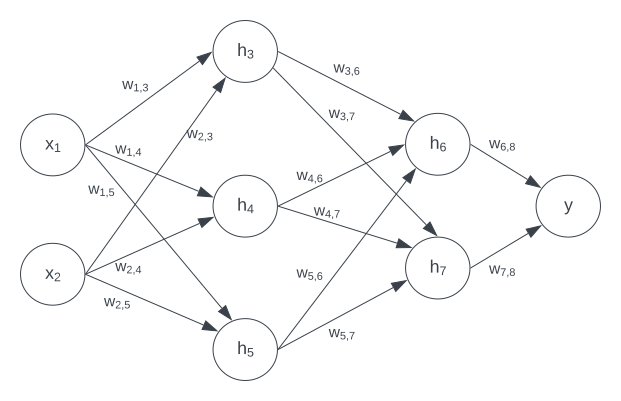
\includegraphics[
        width=12cm,
        keepaspectratio,
    ]{chapters/4. Kuenstliche Neuronale Netze/images/neuronalesnetz}
    \caption{Exemplarische Darstellung der Architektur eines einfachen Feed-Forward-Netzes. (Quelle: Eigene Darstellung)
    \label{fig:multilayerfeedforward}
    \end{center}
    \small{
        Ein Feed-Forward-Netz mit zwei Eingabeeinheiten $x_1, x_2$, zwei versteckten Schichten und einer Ausgabeeinheit $y$. Das dargestellte Netz ist vergleichsweise klein. Grosse Modelle wie Microsoft's Turing-NLG besitzen bis zu $105$ Schichten und $530.000.000.000$ Parameter (\url{https://www.microsoft.com/en-us/research/blog/using-deepspeed-and-megatron-to-train-megatron-turing-nlg-530b-the-worlds-largest-and-most-powerful-generative-language-model/}, abgerufen 27.09.2023).
    }
\end{figure}



\subsection{Backpropagation}\label{sec:backpropagation}
\textit{Murtagh} zeigt in~\cite[185 f.]{Mur91} ein MLP, das mittels \textbf{Backpropagation}\footnote{
    ``das meist genutzte neuronale Modell``~\cite[313]{Ert21b}
} Daten klassifiziert, die keinen linearen Zusammenhang besitzen.
Der Algorithmus geht auf \textit{Rumelhart, Hinton und Williams} zurück, die in~\cite[318 ff.]{RM87} eine Methode\footnote{
    ``The ability to create useful new features distinguishes back-propagation from earlier, simpler methods such as the perceptron-convergence procedure.``~\cite[533]{RHW86}
} vorstellen, um berechnete Werte \textit{rückwärts} in das Netz einzuspeisen.
Hierbei wird für die Netzausgabe (\textit{forward pass}) ein Approximationsfehler berechnet, der als Basis für die Gewichtsänderungen beim rückwärtigen Lauf (\textit{backward pass}) bis zur ersten verborgenen Schicht genutzt wird.
Der Vorgang (forward pass, backward pass, forward pass...) wird so lange für alle Trainingsbeispiele wiederholt, bis die Gewichte sich nicht mehr ändern, oder eine andere Schranke (wie bspw. Epoche oder Zeit) erreicht ist (vgl.~\cite[315]{Ert21b})\footnote{
    ausführlicher Algorithmus in~\cite[853, Abbildung 18.24]{RN09}.
}.



Die mathematische Basis für Backpropagation ist das \textbf{Gradientenabstiegsverfahren}, das dabei hilft, in einem neuronalen Netz Parameter für möglichst optimale (d.h. kleine) Verlust-Werte (also geringe Fehler-Werte) zu finden (vgl.~\cite[837]{RN09}; s. a. Abbildung~\ref{fig:gradient}).
Als Aktivierungsfunktion unterstützt eine \textbf{Sigmoid}-Funktion (Gleichung~\ref{eq:gl-sigmoid} sowie Abbildung~\ref{fig:sigmoid}) aufgrund ihres nicht-linearen Charakters eine größere Klasse darstellbarer Funktionen und damit Lösungen für Probleme, die ein klassisches Perzeptron nicht lösen kann (vgl.~\cite[316]{Ert21b}).\\

Sigmoid:
\begin{equation}
\sigma(x) = \begin{matrix}1 \\ \hline 1 + e^{-x}\end{matrix}
\label{eq:gl-sigmoid}
\end{equation}


\begin{figure}[h]
    \centering
    \includegraphics[
        width=16cm,
        keepaspectratio,
    ]{chapters/4. Kuenstliche Neuronale Netze/images/sigmoid}
    \caption{Plot einer Sigmoid-Funktion. (Quelle: Eigene Darstellung)}
    \label{fig:sigmoid}
\end{figure}


\begin{figure}[h]
    \begin{center}
    \includegraphics[
        width=10cm,
        keepaspectratio,
    ]{chapters/4. Kuenstliche Neuronale Netze/images/gradientenabstieg}
    \caption{Skizzierung des Zusammenhangs Fehlerfunktion und lokale Minima (Quelle: in Anlehnung an~\cite[52, Abb. 2.15]{Son22})}
    \label{fig:gradient}
    \end{enter}
    \small{
     Die $y$-Achse repräsentiert den Fehlerwert, die $x$-Achse den berechneten Gewichtsvektor $w_1$ in einem neuronalen Netz. Offensichtlich existiert in dem Netz $w^*$, für den der Fehler geringer ist als für $w_1$. Das Gradientenabstiegsverfahren wird genutzt, um diese Minima zu finden (vgl.~\cite[52]{Son22}).
}
\end{figure}


\subsection{Neocognitron}

Unter dem Namen \textit{Cognitron} 1975 beschreibt \textit{Fukushima} in~\cite{Fuk75} ein mehrschichtiges Netz mit selbst-organisierenden Eigenschaften zur Mustererkennung, in dem Zellen selektiv auf häufig präsentierte Merkmale reagieren.
1983 veröffentlichen \textit{Fukushima et al.} eine Modifikation dieser Architektur in~\cite{FMI83}\footnote{
    mit Bezug auf~\cite{Fuk80} (``Neocognitron: A self-organizing neural network model for a mechanism of pattern recognition unaffected by shift in position``).
} unter dem Namen \textbf{Neocognitron}\footnote{
    Video mit Demonstration des Netzes unter \url{https://www.youtube.com/watch?v=Qil4kmvm2Sw}, abgerufen 04.09.2023
}; sein biologisches Vorbild ist das durch \textit{Hubel und Wiesel} in~\cite{HW62} beschriebene hierarchische Modell des Wahrnehmungssystems (vgl.~\cite[827]{FMI83}).
In dem künstlichen neuronalen Netz haben Zellen in tiefer liegenden Schichten die Eigenschaft, selektiv komplexere Merkmale der Stimuli zu extrahieren, womit sie weniger anfällig gegenüber Rauschen in den Eingabedaten sind.
In~\cite{Fuk80} war der Trainingsprozess durch wiederholte Einspeisung von Mustern ohne weitere Information gegeben (vgl. ~\cite[197]{Fuk80})\footnote{
    ``learning without a teacher``, also unüberwachtes Lernen (unsupervised learning).
}: Die Erweiterung des Modells beinhaltet nun die Verstärkung der modifizierten Synapsen durch überwachtes Lernen, um bessere Resultate bei handgeschriebenen Zeichen zu erzielen (vgl. ~\cite[829]{FMI83}).
\textit{Anderson und Rosenfeld} attestieren dem Netz von \textit{Fukushima et al.} Aspekte, die bei der Entwicklung neuronaler Netze eine wesentliche Rolle spielen werden (siehe ~\cite[524]{AR88}):  Tatsächlich inspiriert das Neocognitron die Convolutional Neural Networks (CNN) (vgl.~\cite[439]{LBH15}), deren erster Entwurf 1989 von \textit{LeCun} in ~\cite{Cun89} vorgestellt wird.



\subsection{Convolutional Neural Networks}\label{cnn}

\textit{Yann LeCun} veröffentlicht 1989 seine Arbeit~\cite{Cun89}, in der er verschiedene Netzwerkarchitekturen auf Generalisierungsfähigkeit (s. Abschnitt~\ref{sec:lernregel}) und Performance untersucht. Er kommt zu dem Schluss, dass eine Reduzierung der \textit{freien Parameter}\footnote{
    \textit{freie Parameter} sind die Parameter des Netzes, die durch den Lernvorgang festgelegt werden, also bspw. die Gewichte, Schwellenwerte oder auch die Lernrate, wenn diese durch Verwendung bestimmter Optimierungsalgorithmen adaptiv ist, wie bspw. \textbf{Adam} (vgl.~\cite[346]{GBC18} mit Verweis auf~\cite{KB17})
} in einem mehrschichtigen Netz zu einer hohen Generalisierungsfähigkeit führt: Bessere Ergebnisse im Vergleich zu  ein- bzw. zweischichtigen Netzen können erzielt werden, indem sog. \textit{feature maps} genutzt werden, die in den Schichten für die Merkmalsextraktion der Eingabedaten (hier: zweidimensionale Bilder) verantwortlich sind.
Zusätzliche Information wie die Lage der Merkmale in den Eingabedaten werden näherungsweise gespeichert, was zu einer Reduzierung der Größe der \textit{feature maps} im Vergleich zu der Größe der Eingabedaten führt, und damit auch zu einer Reduzierung der Gewichte.
Darüber hinaus können mehrere feature maps die gleichen Merkmale an unterschiedlichen Orten (\textit{shift invariance}) in den Eingabedaten extrahieren, wodurch die Gewichte unter diesen feature maps geteilt werden können (vgl.~\cite[151 f.]{Cun89}).
In~\cite{CBD+89} stellen \textit{LeCun et al.} diese Architektur als \textbf{Convolutional Network} \textit{LeNet-1} vor (vgl.~\cite[13]{CBBH98}), das äußerst erfolgreich mittels Backpropagation handgeschriebene Postleitzahlen erkennt. Das Netz performt mit 30 Klassifizierungen pro Sekunde, lediglich die Normalisierung der Eingabedaten stellt einen Flaschenhals bei dem Prozess dar. Wird dieser berücksichtigt, werden 10-12 Ergebnisse pro Sekunde erzielt (vgl.~\cite[549]{CBD+89}).\\



Eine mathematische Basis von CNNs ist die \textbf{Faltungsoperation}: Hierbei wird auf Eingabedaten ein \textbf{Kernel} (die \textit{Faltungsmatrix})\footnote{
    ``das biologische Analogon zu den Filtern [Kerneln] sind die bei den Sinnesorganen vorkommenden rezeptiven Felder.``~\cite[326]{Ert21b}. Vgl. hierzu auch~\cite[439]{LBH15}.
} angewendet, wobei das Ergebnis der Faltungsoperation die \textbf{feature map} (\textit{Merkmalskarte}) ist (vgl.~\cite[370]{GBC18}). \textit{Goodfellow et al.} erläutern in~\cite[374 ff.]{GBC18} die Optimierungen, die durch den Einsatz von Faltung hervorgehen: Durch den Einsatz von Kerneln, die nur aus einem Bruchteil der Größe der Eingabedaten bestehen\footnote{\textit{Goodfellow et al.} beziffern für Eingaben von 1.000.000 Pixeln Kernel mit einer Grösse von einigen hundert Pixeln als ausreichend (siehe~\cite[374]{GBC18}).
}, können ``aussagekräftige Merkmale`` aufgespürt werden, was dazu führt, das weniger Parameter gespeichert werden müssen und gleichzeitig die ``statistische Effizienz`` des Netzes erhöht wird (\textbf{sparse interaction} bzw. \textbf{sparse weights}). Durch \textbf{parameter sharing} (auch: \textbf{tied weights}) kann die Effizienz des Netzes erhöht und Speicherplatzverbrauch verringert werden, und Schichten weisen eine \textbf{Äquivarianz} gegenüber Verschiebung auf.



\begin{figure}[h]
    \begin{center}
    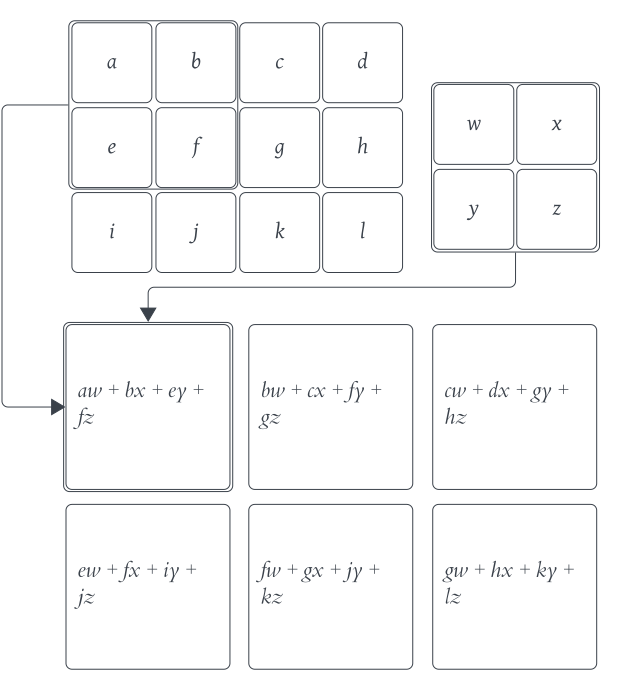
\includegraphics[
        width=10cm,
        keepaspectratio,
    ]{chapters/4. Kuenstliche Neuronale Netze/images/faltung}
    \caption{Beispiel einer Faltungsoperation. (Quelle: in Anlehnung an~\cite[372, Abbildung 9.1]{GBC18})}
    \label{fig:faltung}
    \end{center}
    \small{
    In dem Beispiel wird zur Faltung ein $2 \times 2$-Kernel mit einer $3 \times 4$-Eingabe verwendet. Das Ergebnis ist eine $2 \times 3$-\textit{feature map}.
    }
\end{figure}



CNNs nutzen neben den Convolution Schichten auch Pooling Schichten (vgl.~\cite[325]{Ert21b}), die die Ausgaben des Netzes durch eine ``statistische Größe der nahegelegenen Ausgaben`` ersetzt~\cite[379]{GBC18}, was die Zahl der Pixel auf den feature maps reduziert\footnote{ \textit{LeCun et al.} weisen darauf hin, dass die Pooling Schicht auch die Aufgabe hat, semantisch ähnliche Merkmale zusammenzufassen: ``the role of the pooling layer is to merge semantically similar features into one.``~\cite[439]{LBH15}
}, außerdem wird als Aktivierungsfunktion meistens die nichtlineare ReLu (Rectified Linear Unit, s. Gleichung~\ref{eq:gl-relu} und Abbildung~\ref{fig:relu}) verwendet, die die Konvergenz der Netze verbessert (vgl.~\cite[327]{Ert21b}).\\

ReLU:
\begin{equation} f(x) = max(0, x)
    \label{eq:gl-relu}
\end{equation}


\begin{figure}[h]
    \centering
    \includegraphics[
        width=12cm,
        keepaspectratio,
    ]{chapters/4. Kuenstliche Neuronale Netze/images/relu}
    \caption{Plot der ReLU. (Quelle: Eigene Darstellung)}
    \label{fig:relu}
\end{figure}




